\chapter[Progettazione \texttt{BdD} \& modello \texttt{ER}]{Principi di Progettazione di Basi di Dati e Modello \texttt{ER}}
\thispagestyle{chapterInit}
\label{ch:IlModelloER}
In fase di progettazione della base di dati ci si deve porgere come obbiettivi quelli di:
\begin{itemize}
    \item garantire un alto livello di qualità dei dati memorizzati (anche a lungo termine)
    \item garantire la coerenza con le applicazioni che accedono ai dati
\end{itemize}
\paragraph{Le fasi della progettazione}
    La progettazione di una base di dati si divide in tre fasi principali e altre tre di supporto:
    \begin{enumerate}
        \item \textbf{Analisi dei requisiti}: si cerca di capire quali sono i dati che devono essere memorizzati e come essi sono correlati tra loro
        \item \textbf{Progettazione concettuale}: si costruisce un modello concettuale dei dati, indipendente dal DBMS che si intende utilizzare
        \item \textbf{Progettazione logica}: si traduce il modello concettuale in uno schema logico, che tenga conto delle caratteristiche del DBMS
        \item \textbf{Raffinamento}: si cerca di ottimizzare lo schema logico, per garantire prestazioni migliori (eg. normalizzazione)
        \item \textbf{Progettazione livello fisico}: si definiscono le strutture fisiche che ospiteranno i dati
        \item \textbf{Progettazione applicativa e sicurezza}: si definiscono le procedure e le regole di accesso ai dati
    \end{enumerate}
\section{Analisi dei requisiti}
    Come anticipato in precedenza, le prime fasi della progettazione di una base di dati devono essere svolte rispondendosi a domande come:
    \begin{quote}
        Quali sono i dati che devono essere memorizzati?
    \end{quote}
    Il problema è che a questa domanda non possiamo rispondere per intero, in quanto solitamente questa deve essere fatta a quelle persone che andranno ad utilizzare il sistema e/o chi il sistema lo ha commissionato. Questo comporta che il progettista debba avere una buona capacità di ascolto e di sintesi, solitamente infatti le persone con le quali si parla non hanno una visione chiara di cosa vogliono, e spesso non sanno neanche cosa non vogliono, oltre ad una scarsa conoscenza dell'ambito informatico. Ne consegue che qualche volta questi si contraddicono, e il progettista deve essere in grado di intuire correttamente (o almeno sperare di farlo) cosa vogliono realmente.
    \paragraph{Dalla realtà al modello}
        Una volta raccolti i requisiti, viene quindi costruito un modello concettuale (spesso usando il paradigma \texttt{ER}) che rappresenti i dati e le relazioni tra di essi. Questo modello deve essere il più possibile indipendente dal DBMS che si intende utilizzare, in modo da poter essere facilmente trasformato in uno schema logico.
    \paragraph{Il mini-mondo} 
        Il modello concettuale deve rappresentare il cosiddetto \textit{mini-mondo}, ovvero una rappresentazione semplificata del mondo reale, che contiene solo le informazioni rilevanti per il sistema che si intende realizzare. Questo significa che il modello concettuale non deve contenere informazioni superflue, che non siano necessarie per il sistema.
\section{Il modello \texttt{ER}}
    \subsection{Concetti fondamentali}
        Definiamo ora i concetti principali del modello \texttt{ER}:
        \paragraph{Entità (\textit{entity})} un oggetto del mondo reale (o del nostro mini-mondo) che è distinto da tutti gli altri oggetti. Un'entità è caratterizzata da un insieme di attributi che ne descrivono le proprietà.
        \paragraph{Insieme di entità (\textit{entity set})} un insieme di entità dello stesso tipo (eg. insieme di tutti i dipendenti di un'azienda)
        \paragraph{Tipo di entità (\textit{entity type})} definizione a livello intensionale delle entità a cui fanno riferimento diversi insiemi di entità (eg. tipo di entità \texttt{dipendente} \textit{entity sets} \texttt{dipendenti\_amministrativi}, \texttt{dipendenti\_\_} \texttt{tecnici} etc.)
        \paragraph{Attributi (\textit{attributes})} proprietà che descrivono le entità.
        \paragraph{Insieme di valori (\textit{value set}) - tipo di dato (\textit{data type})} insieme di valori che un attributo può assumere (eg. insieme dei numeri interi, insieme delle stringhe etc.)
        \subsubsection{Gli attributi}
            Gli attributi possono essere di diversi tipi:
            \begin{itemize}
                \item \textbf{Semplici}: non possono essere suddivisi in parti più piccole (eg. nome, cognome)
                \item \textbf{Composti}: possono essere suddivisi in parti più piccole (eg. indirizzo, composto da via, numero civico, città etc.)
                \item \textbf{Multi-valore} possono assumere più di un valore (eg. telefono, che può avere più di un numero)
            \end{itemize}
            \paragraph{Attributi chiave} Esistono degli attributi speciali, chiamati \textbf{chiave}, che permettono di identificare univocamente un'entità, come ad esempio il codice fiscale, il codice di un dipendente etc. Ogni \textit{entity type} deve uno o un insieme di attributi che lo identifichino univocamente, questo/i attributo/i è/sono chiamati attributo/i chiave.
            \subparagraph{Più chiavi} Un'entità può avere più di una \textbf{chiave candidata} (ovvero un insieme di attributi che identificano univocamente un'entità), una di queste verrà scelta come chiave primaria.\newline \underline{Nel modello \texttt{ER} la chiave primaria è sempre sottolineata.}
        \paragraph{Rappresentazione \textit{Entity type}} Un \textit{entity type} viene rappresentato con un rettangolo, con il nome dell'entità al suo interno. Gli attributi vengono rappresentati con un ovale, con il nome dell'attributo al suo interno. La chiave primaria viene sottolineata.
            \begin{figure}[H]
                \centering
                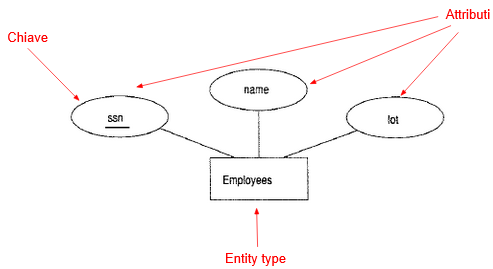
\includegraphics[width=0.5\textwidth]{04/ER-type.png}
                \caption{Rappresentazione di un \textit{entity type}}
            \end{figure}
    \subsection{Primo Raffinamento: le relazioni (\textit{relationships})}
        Si introducono dopo una prima fase di progettazione le relazioni. Una relazione (\textit{relationship}) è un'associazione tra due o più entità, come ad esempio l'associazione tra un dipendente e il suo dipartimento. Le relazioni dello stesso gruppo vengono raggruppate in un \textit{relationship set}. Il numero di \textit{entity type} che partecipano ad un \textit{relationship type} si dice \textbf{grado} della relazione.
        \paragraph{Attributi descrittivi}
            Una relazione può avere degli attributi che la descrivono, come ad esempio la data di inizio di un rapporto di lavoro tra un dipendente e un dipartimento. Gli attributi di una relazione forniscono solo informazioni su quella relazione, e \textbf{non} sulle entità che vi partecipano. Per questo motivo una relazione è identificata univocamente dalle entità che vi partecipano e \textbf{non} dagli attributi descrittivi.
        \paragraph{Relazioni ternarie} Come anticipato, una relazione può coinvolgere più di due \textit{entity type}, in tal caso si parla di relazione ternaria, quaternaria etc\dots In questo caso non avremo più solo due attributi che identificano la relazione, ma tre, quattro etc\dots Per il resto il concetto rimane invariato.
        \paragraph{Esempio} si consideri il seguente esempio di schema \texttt{ER}:
            \begin{figure}[H]
                \centering
                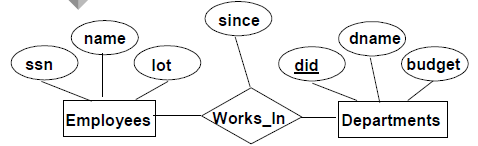
\includegraphics[width=0.5\textwidth]{04/ER-relations.png}
                \caption{Esempio di relazione tra due \textit{entity type}}
            \end{figure}
            Nell'esempio in figura la relazione "\texttt{Works\_In}" è di grado 2, in quanto coinvolge due \textit{entity type} (\texttt{Employees} e \texttt{Departments}).\newline
            Si noti come per una coppia degli attributi \texttt{<ssn, did>} si possa avere al massimo un solo valore per l'attributo \texttt{since} (ovvero la data di inizio del rapporto di lavoro tra un dipendente e un dipartimento).
        \paragraph{\textit{Relationship type} vs. \textit{relationship set}} Un \textit{relationship type} è lo schema che descrive la relazione, ne identifica il nome e gli \textit{entity types} che vi partecipano, infine identifica i vincoli associati ad essa. Un \textit{relationship set} è un insieme di istanze della relazione, rappresentate nella base di dati, con un parallelismo improprio e informale: "il \textit{relationship set} è lo stato attuale di un \textit{relationship type}".
    \subsection{Vincoli sulle relazioni}
        Distinguiamo in una relazione i seguenti vincoli:
        \begin{itemize}
            \item Vincoli di chiave (\textit{key constraints})
            \item Vincoli di cardinalità (\textit{cardinality ratio})
            \item Vincoli di esistenza o partecipazione (\textit{participation constraints})
        \end{itemize}
        \subsubsection{Vincoli di chiave}
            I vincoli di chiave permette di esprimere la condizione secondo la quale una entità possa partecipare al massimo una volta ad una relazione. Questo vincolo è espresso tramite una freccia con la punta annerita che parte dall'entità che può partecipare al massimo una volta e punta verso la relazione.
            \begin{figure}[H]
                \centering
                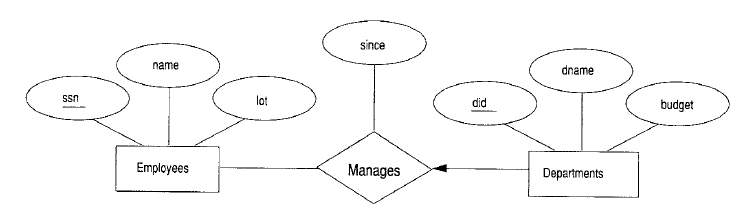
\includegraphics[width=0.5\textwidth]{04/ER-key-constraint.png}
                \caption{Vincolo di chiave}
            \end{figure}
            Nell'esempio: un dipartimento può avere al massimo un \textit{manager} (ovvero un dipendente), ma un dipendente può essere \textit{manager} anche di più dipartimenti.\newline
            Stessa cosa valer per le relazioni con grado maggiore di 2, per cui ad esempio un dipendente può lavorare su una sola sede di un dipartimento ma una sede può avere più dipendenti e un dipartimento può avere più sedi.
        \subsubsection{Vincoli di cardinalità}
            Servono a esprimere il numero \textbf{massimo} di volte che un'entità può \textbf{comparire} \footnote{Si noti che il vincolo di cardinalità non esprime il numero di volte che un'entità può partecipare ad una relazione, ma il numero di volte che un'entità può comparire in un \textit{relationship set}.} in un \textit{relationship set}. Questi vincoli sono espressi tramite una coppia di numeri, che indicano rispettivamente il numero minimo e massimo di volte che un'entità può comparire in un \textit{relationship set}.\newline
            Solitamente sono rappresentati ed espressi come:
            \begin{itemize}
                \item \textit{One-to-One} (1:1)
                \item \textit{One-to-Many} (1:N) o \textit{Many-to-One} (N:1)
                \item \textit{Many-to-One} (N:1)
            \end{itemize}
            Questi sono posti in prossimità della relazione, e sono separati da un trattino.
        \subsubsection{Vincoli di partecipazione}
            I vincoli di partecipazione specificano quante volte un'entità deve comparire \textbf{al minimo} in una relazione, per questi vincoli sono detti anche \textit{Existence Dependency Constraints}. 
            % TODO Finire la sotto-sotto-sezionle